\subsubsection{ Digit readers }

\begin{itemize}

\item For each $i = 1,2,3$,
               $j = 0,\ldots,l-3$,
               $u \in \{0, 1\}^j$, and
               $\inc \in \{{\tt increment}, {\tt copy} \}$:
    \begin{itemize}
        \item if $j = 0$:
        create
        $\begin{aligned}[t]
            \cread(& \left\langle {\tt Read}, i, \lambda, \inc \right\rangle,
                     \left\langle {\tt Read}, i, 0, \inc \right\rangle,
                     \left\langle {\tt Read}, i, 1, \inc \right\rangle \;)
        \end{aligned}$\\ from the general gadget in Figure~\ref{fig:counter_read}.

        \item else:
        create
        $\begin{aligned}[t]
        \cread(& \left\langle {\tt Read}, i, u,  \inc \right\rangle,
                 \left\langle {\tt Read}, i, 0u, \inc \right\rangle,
                 \left\langle {\tt Read}, i, 1u, \inc \right\rangle \;)
        \end{aligned}$\\ from the general gadget in Figure~\ref{fig:counter_read}.
    \end{itemize}

\end{itemize}

% Might be off by one?

\begin{itemize}

    \item For each $i = 1,2,3$ and each $u \in \{0, 1\}^{l-2}$:

    \begin{itemize}
        \item Create $\begin{aligned}[t]
            \cread(& \left\langle {\tt Read},    i,  u, {\tt copy} \right\rangle,
                     \left\langle {\tt PreWarp}, i, 0u, {\tt copy} \right\rangle,
                     \left\langle {\tt PreWarp}, i, 1u, {\tt copy} \right\rangle \;)
        \end{aligned}$\\from the general gadget in Figure~\ref{fig:counter_read}.
    \end{itemize}
\end{itemize}

Since the counter must only increment the current value if the result will be less than $m$,
the \\{\cread} gadgets that have both an {\tt increment} signal and input size of $l - 2$ must
first right shift the bits 2 spots, and then for each possible value after reading one more bit,
check whether that value is less than $m - 1$. Basically, if the next bit read is a 0, we check
if the current value + 1 is less than $m$. If the next bit read is a 1, we check if current value +
$2m + 1$ is less than $m$. For both cases, if the counter can increment the current value, then
the {\cread} gadgets output the incremented value to the {\prewarp} gadgets and propagate a {\tt copy}
signal. Otherwise, if the counter is unable to increment the value, it outputs a digits with all
zeroes and propagates the {\tt increment} signal to the next digit.

\begin{itemize}

    \item For each $i = 1,2,3$ and each $u \in \{0, 1\}^{l-2}$:

    Let $guess0$ = $0u >> 2$, $guess1$ = $1u >> 2$

    \vspace{.5cm}
    if $dec(guess0) + 1 < m - 1$

    % convert the result to binary and re-add the least signifcant two bits
    then $R0$ = $bin(dec(guess0) + 1)+u[1]+u[0], {\tt copy}$

    else $R0$ = $\{0 \}^l, {\tt increment}$

    \vspace{.5cm}

    if $dec(guess1) + 1 < m - 1$

    % convert the result to binary and re-add the least signifcant two bits
    then $R1$ = $bin(dec(guess1) + 1)+u[1]+u[0], {\tt copy}$

    else $R1$ = $\{0 \}^l, {\tt increment}$

    \vspace{.5cm}

    \begin{itemize}
        \item Create
        $\begin{aligned}[t]
            \cread(& \left\langle {\tt Read},    i,  u, {\tt increment} \right\rangle,
                     \left\langle {\tt PreWarp}, i, R0                  \right\rangle,
                     \left\langle {\tt PreWarp}, i, R1                  \right\rangle \;)
        \end{aligned}$\\from the general gadget in Figure~\ref{fig:counter_read}.
    \end{itemize}

\end{itemize}

\begin{figure}[H]
    \centering
    \begin{subfigure}[t]{0.2\textwidth}
        \centering
        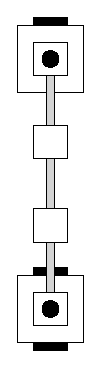
\includegraphics[width=0.2\textwidth]{counter_read_0}
        \caption{\label{fig:counter_read_0} {\tt Counter\_Read\_0}}
    \end{subfigure}%
    ~
    \begin{subfigure}[t]{0.2\textwidth}
        \centering
        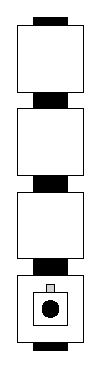
\includegraphics[width=0.2\textwidth]{counter_read_1}
        \caption{\label{fig:counter_read_1} {\tt Counter\_Read\_1}}
    \end{subfigure}%
    \caption{\label{fig:counter_read} The {\tt Counter\_Read} gadgets}
\end{figure}
